\section{Superfluid Æther Framework}

We assume a stationary Euclidean 3-dimensional æther that behaves as a superfluid-like medium with zero viscosity and constant mass density.\ This continuous medium forms the basis of all physics: particles are topological vortex structures in the æther and fields correspond to flow patterns (vorticity, pressure, etc.). The dynamics are governed by classical flow equations, with the following fundamental postulates:

\vspace{1em}
\subsection*{Ætheric Pressure and Density Notation}

\paragraph{Ætheric Pressure \textbf{\( p \)}:}
In classical fluids, pressure arises from random molecular collisions.\ In the æther model,  \textbf{\( p \)} refers instead to an effective stress field arising from compressional or circulatory æther motion.\ It represents momentum flux across surfaces and governs how flow gradients influence acceleration.\ Specifically, the force density on a fluid element is given by the Euler relation:
\[
\vec{f} = -\frac{\nabla p}{\rho^{\text{(fluid)}}_{\text{\ae}}}
\]
Here, pressure is not thermal but a mechanical quantity tied to vortex tension, compressional strain, and the local geometry of flow.

\paragraph{Density Notation:}
In this model, we distinguish two types of æther density:

\begin{itemize}
    \item \textbf{\(\rho^{\text{(fluid)}}_{\text{\ae}}\)} — the background \textbf{fluid mass density} of the æther \([ \text{kg/m}^3 ]\). It appears in hydrodynamic relations such as:
    \[
    c = \sqrt{\frac{B}{\rho^{\text{(fluid)}}_{\text{\ae}}}}, \quad \vec{f} = -\frac{\nabla p}{\rho^{\text{(fluid)}}_{\text{\ae}}}
    \]

    \item \textbf{\(\rho^{\text{(energy)}}_{\text{\ae}}\)} — the \textbf{energy density} of the æther \([ \text{J/m}^3 ]\), which accounts for stored swirl energy, vortex stress, and energy transport capacity.

    \item \textbf{Default convention:} When the symbol \(\rho\) is used without a superscript, it refers to \(\rho^{\text{(fluid)}}_{\text{\ae}}\) by default.

    \item The two are related via:
    \[
    \rho^{\text{(energy)}}_{\text{\ae}} = \frac{1}{2} \rho^{\text{(fluid)}}_{\text{\ae}} c^2
    \]
\end{itemize}

\begin{figure}[htbp]
    \centering
    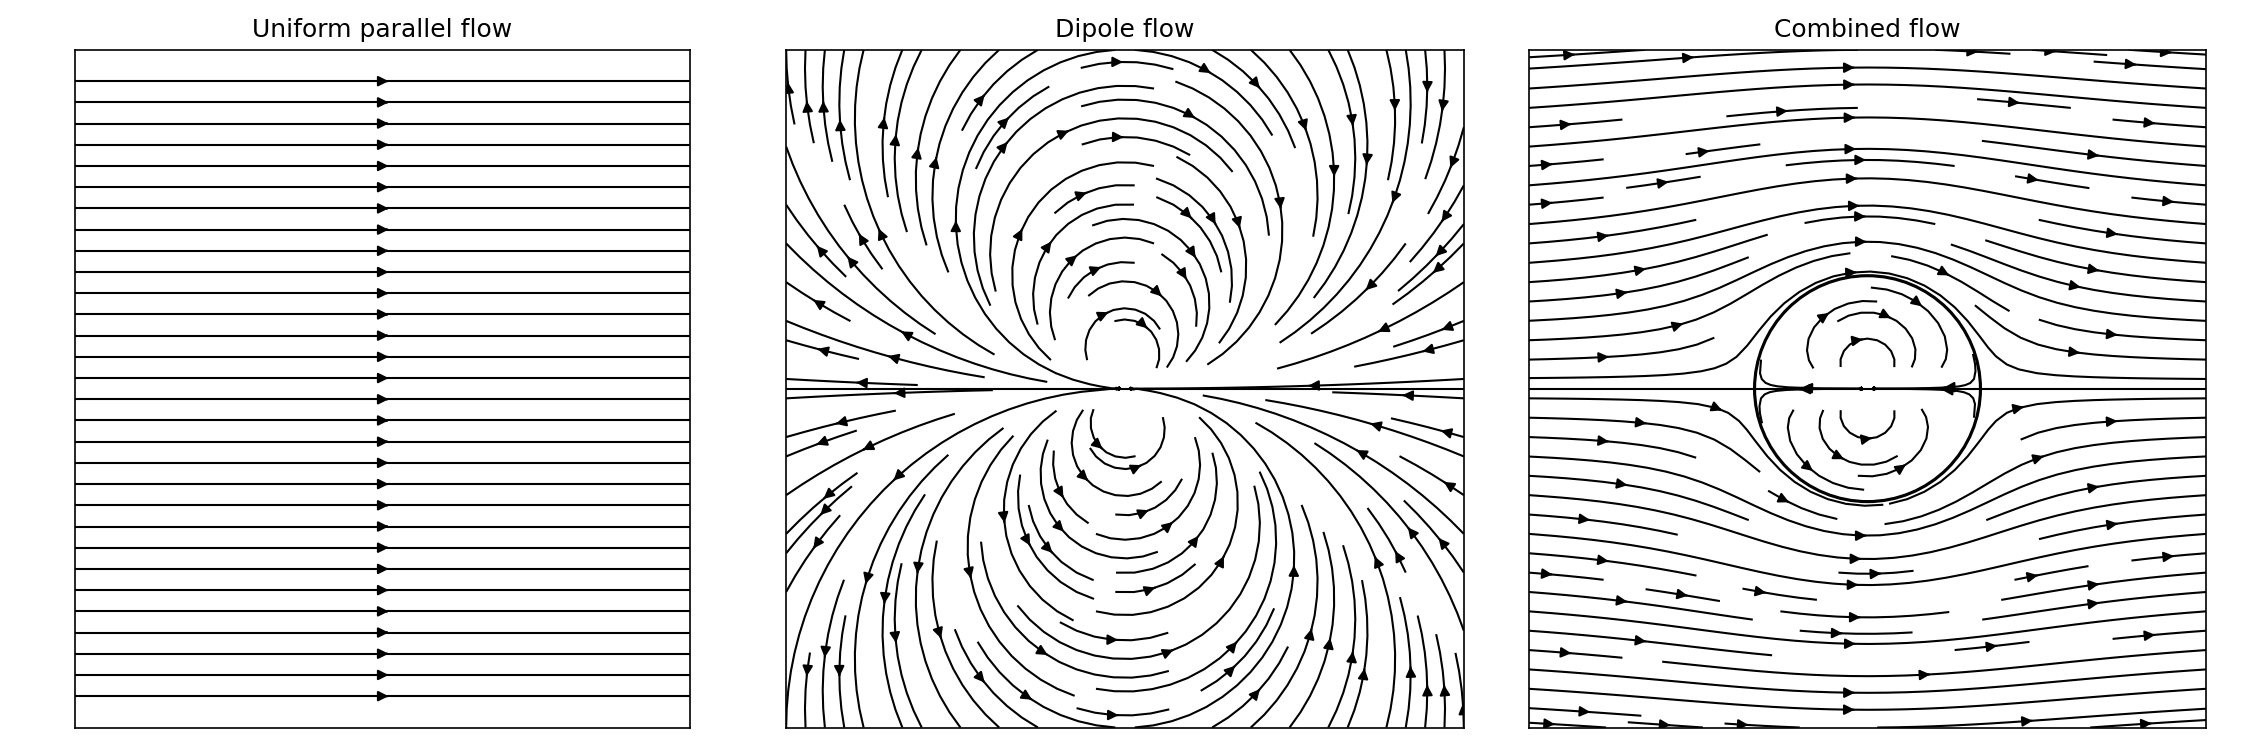
\includegraphics[width=0.85\textwidth]{images/03-combined_flow}
    \caption{Illustration of æther flow and vorticity around vortex cores.}
    \label{fig:vortexfields}
\end{figure}


\begin{description}
    \item[\textbf{Postulate I: Absolute flat space}] \hfill \\
    Space is a stationary, flat Euclidean background with a preferred frame defined by the æther at rest.\ All distances and velocities are measured in it.\ There is no intrinsic spacetime curvature; all metrics are derived from flow fields.\ (This is similar to Lorentz's original absolute frame concept, but now with a physical superfluid-like filling space~\cite{Winterberg2002-PlanckÆther}).

    \item[\textbf{Postulate II: Approximately incompressible uniform æther}] \hfill \\
    The æther behaves as an ideal fluid with zero viscosity and approximately constant mass density \textbf{$\rho^{\text{(fluid)}}_{\text{\ae}}$} in large-scale regions (analogous to superfluid helium at $T=0$). However, compressibility is permitted near vortex cores and in regions of high swirl energy, where local gradients in \textbf{$\rho^{\text{(energy)}}_{\text{\ae}}$} may develop.\ These gradients support field dynamics and mass-energy emergence.\ This scale-dependent compressibility is negligible for low-energy vortical flow but crucial in quantum-scale interactions.

    \item[\textbf{Postulate III: Vortex nodes as matter}] \hfill \\
    Matter particles are modeled as stable, topologically conserved vortex nodes.\ According to Kelvin~\cite{Kelvin1867-vortex}, an atom or fundamental particle is a quantized vortex loop or node in the æther.\ It has a well-defined core (of the order of the Planck length $l_{\textrm P}$ in radius, according to Planck-æther theories~\cite{Winterberg2002-PlanckÆther}) around which æther flows circularly.

    \item[\textbf{Postulate IV: Time as Vortex-Core Rotation}] \hfill \\
    Proper time is defined by the cumulative internal rotations of a vortex core relative to the æther rest frame. Time is not a global coordinate but a local, topological property emerging from rotation.

    To formalize this, we distinguish several temporal constructs:

    \begin{itemize}
        \item $\boldsymbol{\mathcal{N}}$ — absolute æther time (Aithēr-Time)
        \item $\boldsymbol{\tau}$ — local measurable proper time (Chronos-Time)
        \item $\boldsymbol{\mathcal{S}(t)}$ — swirl clock phase for vortices
        \item $\boldsymbol{T_v}$ — proper time around a vortex loop (Vortex-Time)
        \item $\boldsymbol{\mathbb{K}}$ — kairotic moment: emergent threshold events
    \end{itemize}

    These layers allow precision in expressing time dilation, identity coherence, and synchronization phenomena. (See Appendix~\ref{appendix:temporal_structures} for full table.)

    All particles evolve within the same ætheric Now, denoted by $\boldsymbol{\nu_0}$ — a universal temporal slice in the æther frame $\boldsymbol{\Xi_0}$. Local clocks measure their evolution via $\boldsymbol{\mathcal{S}(t)}$, where:
    \[
    \mathcal{S}(t)_{\circlearrowleft} \quad \text{(vortex)} \qquad \mathcal{S}(t)_{\circlearrowright} \quad \text{(antivortex)}
    \]

    Time dilation thus emerges from disparities in local swirl energy or core circulation, yielding phase mismatches across identical ætheric backgrounds. Two particles can share the same ætheric Now, $\boldsymbol{\nu_0}$, while their $\tau$ or $\mathcal{S}(t)$ progress at different rates.

    At critical moments — resonance, phase-locking, decay — dynamics are governed by the irreversible kairotic time $\boldsymbol{\mathbb{K}}$, which marks discrete transitions rather than continuous flows.


    \item[\textbf{Postulate V: Thermodynamics as Emergent Behavior}] \hfill \\
    Thermal phenomena arise not from the fundamental æther itself, but from statistical interactions among its vortical excitations. The æther is inherently cold, inviscid, and non-dissipative; temperature and entropy emerge as macroscopic averages over microscopic swirl fluctuations. This aligns with the interpretation of thermodynamic irreversibility as a collective vortex phase dispersion.

    \item[\textbf{Postulate VI: Forces via Vorticity Fields}] \hfill \\
    All classical forces are modeled as effective manifestations of ætheric vorticity. Gravitational and electromagnetic fields correspond to structured circulation patterns within the medium. The \textbf{maximum force principle},
    \[
    \boldsymbol{F^{\text{max}}_{\text{gr}} = \frac{c^4}{4G}},
    \]
    represents the æther’s upper limit for stress propagation, interpreted as the peak swirl tension transmissible through the medium.

    \item[\textbf{Postulate VII: Vorticity Conservation and Topology}] \hfill \\
    The total vorticity $\boldsymbol{\vec{\omega}}$ is conserved along flow lines unless reconnection events or external forces intervene. This conservation governs knot topology, circulation quantization, and vortex stability. The transmission of interactions through vortex loops follows analogues of the Biot–Savart law, enabling long-range influence without invoking fields as fundamental.~\cite{helmholtz1858vortices}.
\end{description}


\subsection*{Interpretation: Time as Local Phase in a Shared Now}

In the VAM, time is locally generated yet globally referenced. Each vortex advances its proper time $\boldsymbol{\tau}$ via rotation, but all are synchronized to the ætheric present $\boldsymbol{\nu_0}$:
\[
\Delta \tau = \omega_1^{-1} N_1 - \omega_2^{-1} N_2
\tag{Vortex Clock Synchronization}
\]

Here, $N_i$ counts full rotations, and $\omega_i$ are angular velocities relative to $\boldsymbol{\mathcal{N}}$. This offers a mechanistic view of relativistic time: a vortex ages more if it spins more.

\begin{remark}
\textbf{On Temporal Ontology:} Rather than a universal ticking clock, we posit a globally synchronized ætheric \emph{Now}, within which vortex-based clocks trace their own $\boldsymbol{\tau}$ and $\boldsymbol{\mathcal{S}(t)}$ through motion and identity.
\end{remark}


\subsection*{Fundamental Constants and Relations}
The Planck time, often interpreted as the fastest meaningful tick of a quantum clock, is:
\[
    t_{\textrm P} = \sqrt{\frac{\hbar G}{c^5}} \approx 5.39\times10^{-44}\ \text{s},
\]
with $l_{\textrm P} \approx 1.62\times10^{-35}$ m the corresponding Planck length.\ In this model, such scales define core vortex radii and rotation periods.

The wave propagation (or signal) speed in the æther is given by:
\[
    c = \sqrt{\frac{B}{\rho^{\text{fluid}}_{\text{\ae}}}},
\]
where $B$ is the bulk modulus and $\rho^{\text{fluid}}_{\text{\ae}}$ is the fluid mass density.\ This governs compressional waves and sets the maximal flow velocity.

Energy density is related to fluid mass density by:
\[
    \rho^{\text{energy}}_{\text{\ae}} = \frac{1}{2} \rho^{\text{fluid}}_{\text{\ae}} c^2.
\]

Finally, the maximum force limit is:
\[
    F^{\text{max}}_{\text{gr}} = \frac{c^4}{4G} \approx 3.0 \times 10^{43}\ \text{N},
\]
which in this model represents the æther’s maximal stress capacity.